\subsection{Caso 8. Escaneo de puertos y fingerprinting de servicios}
\label{caso:escaneo-puertos}

\begin{situacion}
Los registros muestran intentos secuenciales contra varios puertos o servicios no habituales de un servidor de laboratorio.
\textbf{Objetivo:} \par
Reproducir un escaneo de puertos autorizado, medir su huella en la red y en un IDS, identificar los servicios expuestos y proponer una lista de exposición con controles de reducción de superficie y reglas de detección. \par
\textbf{Fundamento teórico:} \par
El escaneo de puertos aprovecha el comportamiento de TCP y UDP para inferir qué servicios escucha un host. En TCP, un escaneo SYN envía un segmento con la bandera SYN: si el puerto está abierto, el servidor responde SYN-ACK; si está cerrado, responde RST. El escaneo no completa el \textit{three-way handshake}, por lo que también se denomina \textit{half-open}. En UDP no existe un handshake equivalente: un puerto cerrado suele responder con ICMP de puerto inalcanzable, mientras que uno abierto puede no responder, lo que produce el estado ambiguo \texttt{open|filtered}. El \textit{fingerprinting} posterior envía sondas específicas por servicio para obtener banners y versiones \parencite{nmap}.
\end{situacion}

\paragraph{Procedimiento.}
El escenario reutiliza la red aislada del Caso 7: analista en \texttt{172.28.50.10} y víctima en \texttt{172.28.50.20}, con servicios FTP, SSH, Telnet, HTTP y dos servicios de prueba. El procedimiento fue:

\begin{enumerate}
	\raggedright
	\item \textbf{Integridad:} se calcularon las huellas SHA-256 de las tres capturas antes de analizarlas (Figura~\ref{fig:c8_hashes}).
	\item \textbf{Escaneo SYN:} se ejecutó \texttt{nmap -sS -Pn -n -p 1-1024 --min-rate 1500 --max-retries 1} y se capturó \texttt{CU8\_01\_syn\_scan.pcap} (Figura~\ref{fig:c8_nmap_syn}).
	\item \textbf{Fingerprinting:} se ejecutó \texttt{nmap -sT -sV -Pn -n -p 21,22,23,80,4444,8080 --version-all} y se capturó \texttt{CU8\_02\_service\_scan.pcap} (Figura~\ref{fig:c8_nmap_svc}).
	\item \textbf{Escaneo UDP:} se ejecutó \texttt{nmap -sU -Pn -n -p 53,123,161,500,5353} y se capturó \texttt{CU8\_03\_udp\_scan.pcap}.
	\item \textbf{Análisis de flujos:} con \texttt{tshark} se contaron paquetes SYN, SYN-ACK y RST, puertos destino únicos, duración y tasa (Figuras~\ref{fig:c8_cobertura} y~\ref{fig:c8_flags}).
	\item \textbf{Validación con IDS:} se reprocesó la captura SYN con Suricata 7.0.7 y las reglas locales (Figura~\ref{fig:c8_suricata}).
\end{enumerate}

\begin{figure}[H]
	\centering
	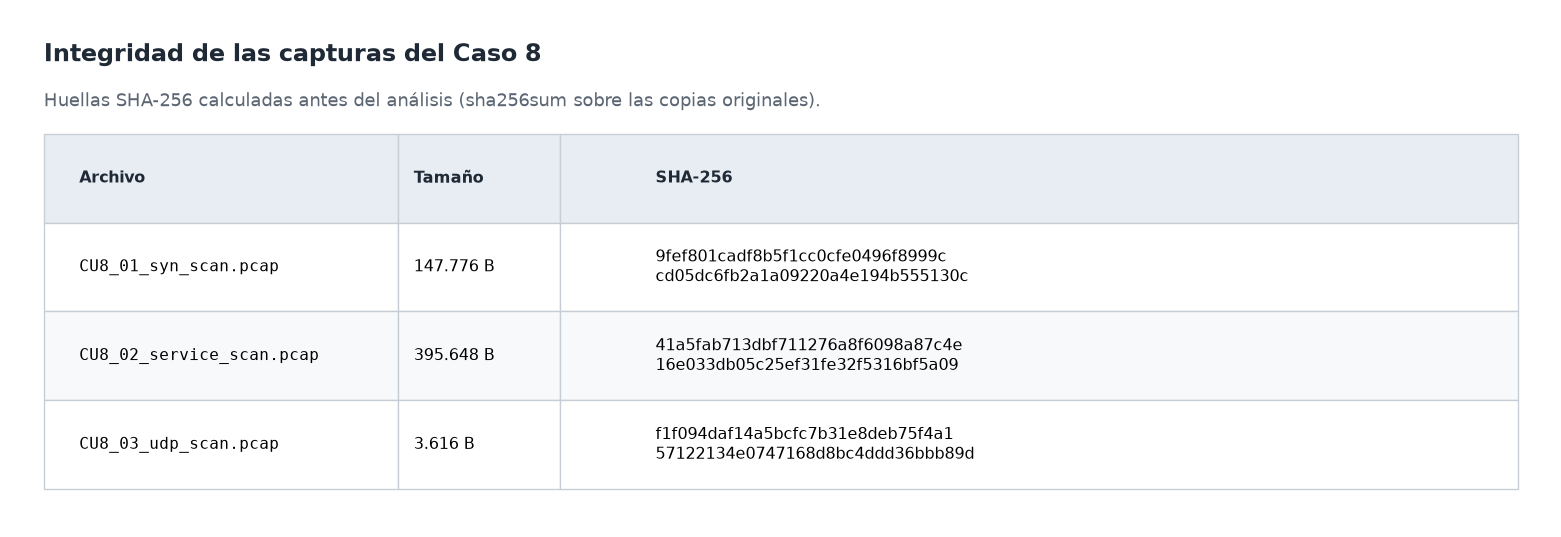
\includegraphics[width=0.92\textwidth]{imagenes/Evidencias CU-8/01_hashes_sha256.png}
	\caption{Verificación de integridad de las capturas del Caso 8 mediante SHA-256.}
	\label{fig:c8_hashes}
\end{figure}

\begin{figure}[H]
	\centering
	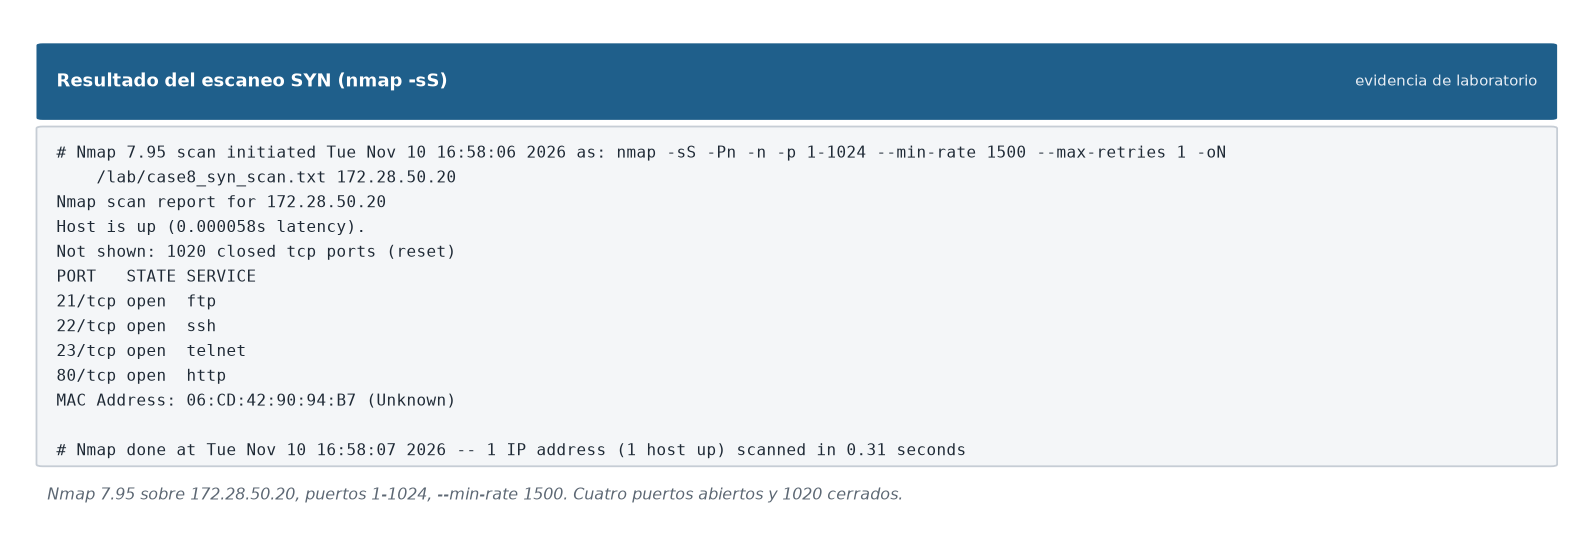
\includegraphics[width=0.98\textwidth]{imagenes/Evidencias CU-8/02_nmap_syn.png}
	\caption{Resultado del escaneo SYN sobre los puertos 1--1024 de la víctima.}
	\label{fig:c8_nmap_syn}
\end{figure}

\begin{figure}[H]
	\centering
	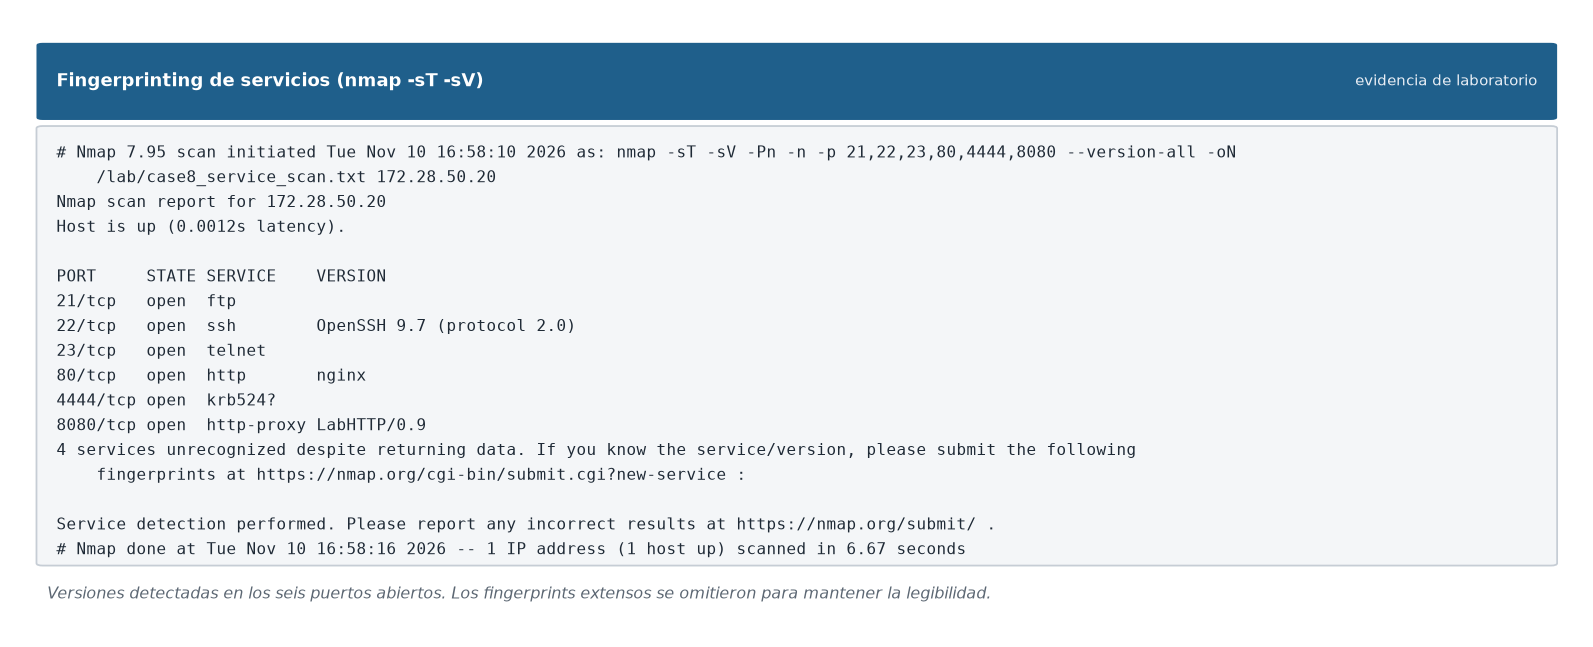
\includegraphics[width=0.98\textwidth]{imagenes/Evidencias CU-8/03_nmap_servicios.png}
	\caption{Detección de versiones y banners de los servicios expuestos.}
	\label{fig:c8_nmap_svc}
\end{figure}

\paragraph{Resultados obtenidos.}
La Tabla~\ref{tab:c8_resumen} resume las métricas de las tres capturas. El escaneo SYN generó 2052 paquetes TCP en 59~ms, con 1024 SYN, 4 SYN-ACK y 1020 RST; es decir, 1024 puertos únicos, de los cuales solo cuatro estaban abiertos (21, 22, 23 y 80). La tasa media fue de aproximadamente 17\,400 SYN por segundo (34\,817 paquetes TCP por segundo si se cuentan también las respuestas).

\begin{table}[H]
	\caption{Métricas de las capturas del Caso 8}
	\label{tab:c8_resumen}
	\centering
	\footnotesize
	\renewcommand{\arraystretch}{1.25}
	\begin{tabularx}{\textwidth}{@{}>{\raggedright\arraybackslash}p{0.26\textwidth} c c c Y@{}}
		\toprule
		\textbf{Captura} & \textbf{Paquetes} & \textbf{Puertos} & \textbf{Duración} & \textbf{Observación} \\ \midrule
		\texttt{CU8\_01\_syn\_scan} & 2052 TCP & 1024 & 59~ms & 1024 SYN, 4 SYN-ACK, 1020 RST. \\ \hline
		\texttt{CU8\_02\_service\_scan} & 4214 TCP & 6 & 6,67~s & 328\,200 bytes; banners y versiones. \\ \hline
		\texttt{CU8\_03\_udp\_scan} & 28 UDP & 5 & 1,75~s & 7 ICMP de puerto inalcanzable. \\
		\bottomrule
	\end{tabularx}
\end{table}

\begin{figure}[H]
	\centering
	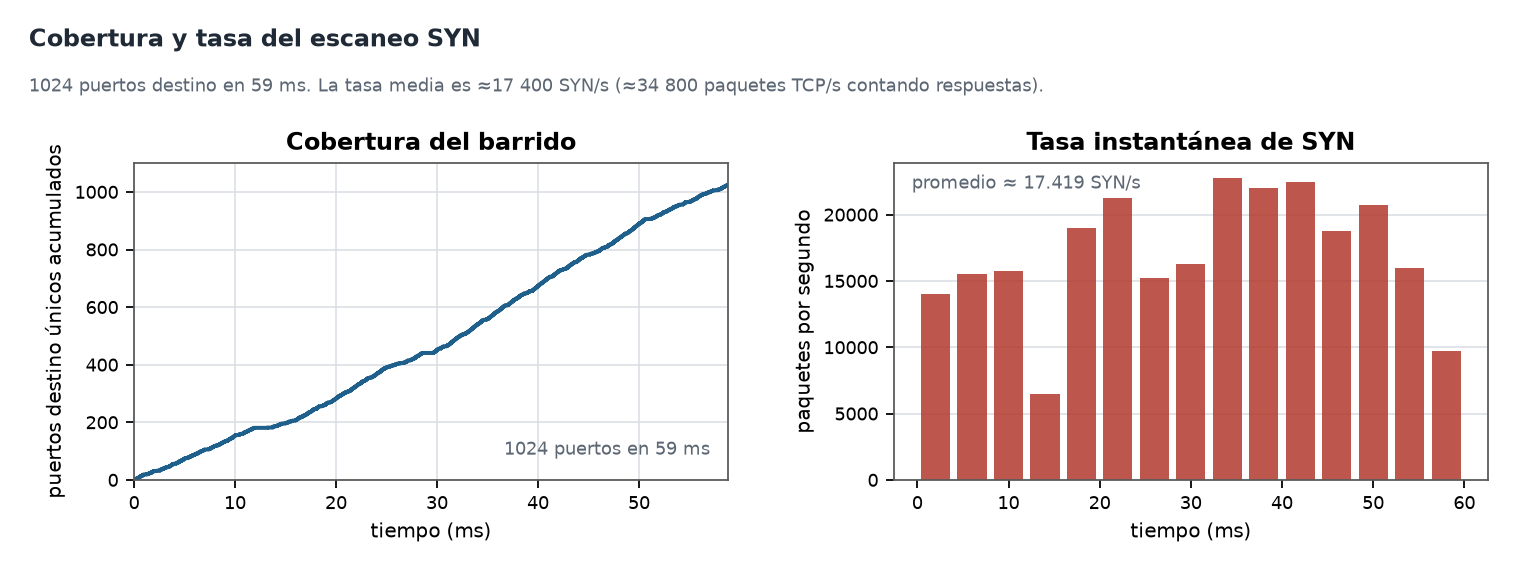
\includegraphics[width=0.98\textwidth]{imagenes/Evidencias CU-8/04_puertos_acumulados.png}
	\caption{Cobertura acumulada de puertos y tasa instantánea del escaneo SYN.}
	\label{fig:c8_cobertura}
\end{figure}

\begin{figure}[H]
	\centering
	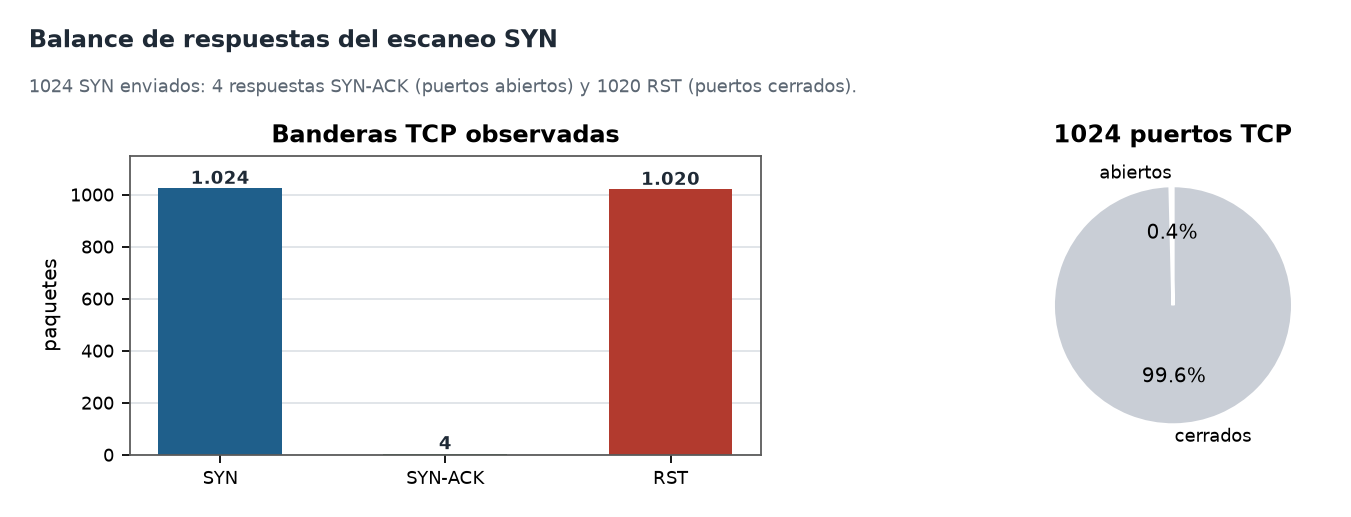
\includegraphics[width=0.92\textwidth]{imagenes/Evidencias CU-8/05_conteo_flags.png}
	\caption{Balance de banderas TCP y proporción de puertos abiertos frente a cerrados.}
	\label{fig:c8_flags}
\end{figure}

\paragraph{Análisis de resultados.}
El escaneo SYN deja una huella muy reconocible: una ráfaga de segmentos SYN con puertos destino crecientes, seguida de RST para los puertos cerrados y de SYN-ACK para los abiertos. La proporción de RST (1020 de 1024 puertos, 99,6\,\%) y la ausencia de un handshake completo confirman el carácter \textit{half-open} del barrido. La tasa instantánea, superior a 20\,000 SYN/s en varios intervalos, es muy superior a la de un cliente legítimo y explica por qué un umbral simple de 30 SYN en 10~s detecta el evento.

El escaneo de servicios, en cambio, sí completa conexiones y solicita banners. Eso permite identificar versiones concretas: OpenSSH~9.7 en el puerto 22, nginx en el 80, \texttt{Laboratorio FTP 1.0} en el 21, \texttt{Laboratorio Telnet 0.9} en el 23 y \texttt{LabHTTP/0.9} en el 8080. El puerto 4444 respondió con \texttt{LAB-SVC/0.1 ready}, un servicio no estándar que Nmap no pudo clasificar y etiquetó como \texttt{krb524?}; esa ambigüedad es una limitación del fingerprinting y, a la vez, una señal de que el servicio no debería estar expuesto sin justificación.

El escaneo UDP fue mucho menos concluyente: 53, 123, 161 y 5353 respondieron con ICMP de puerto inalcanzable (cerrados), mientras que el 500 quedó en \texttt{open|filtered} porque no hubo respuesta. La ausencia de respuesta no prueba que el puerto esté abierto: puede deberse a un filtrado silencioso.

\begin{figure}[H]
	\centering
	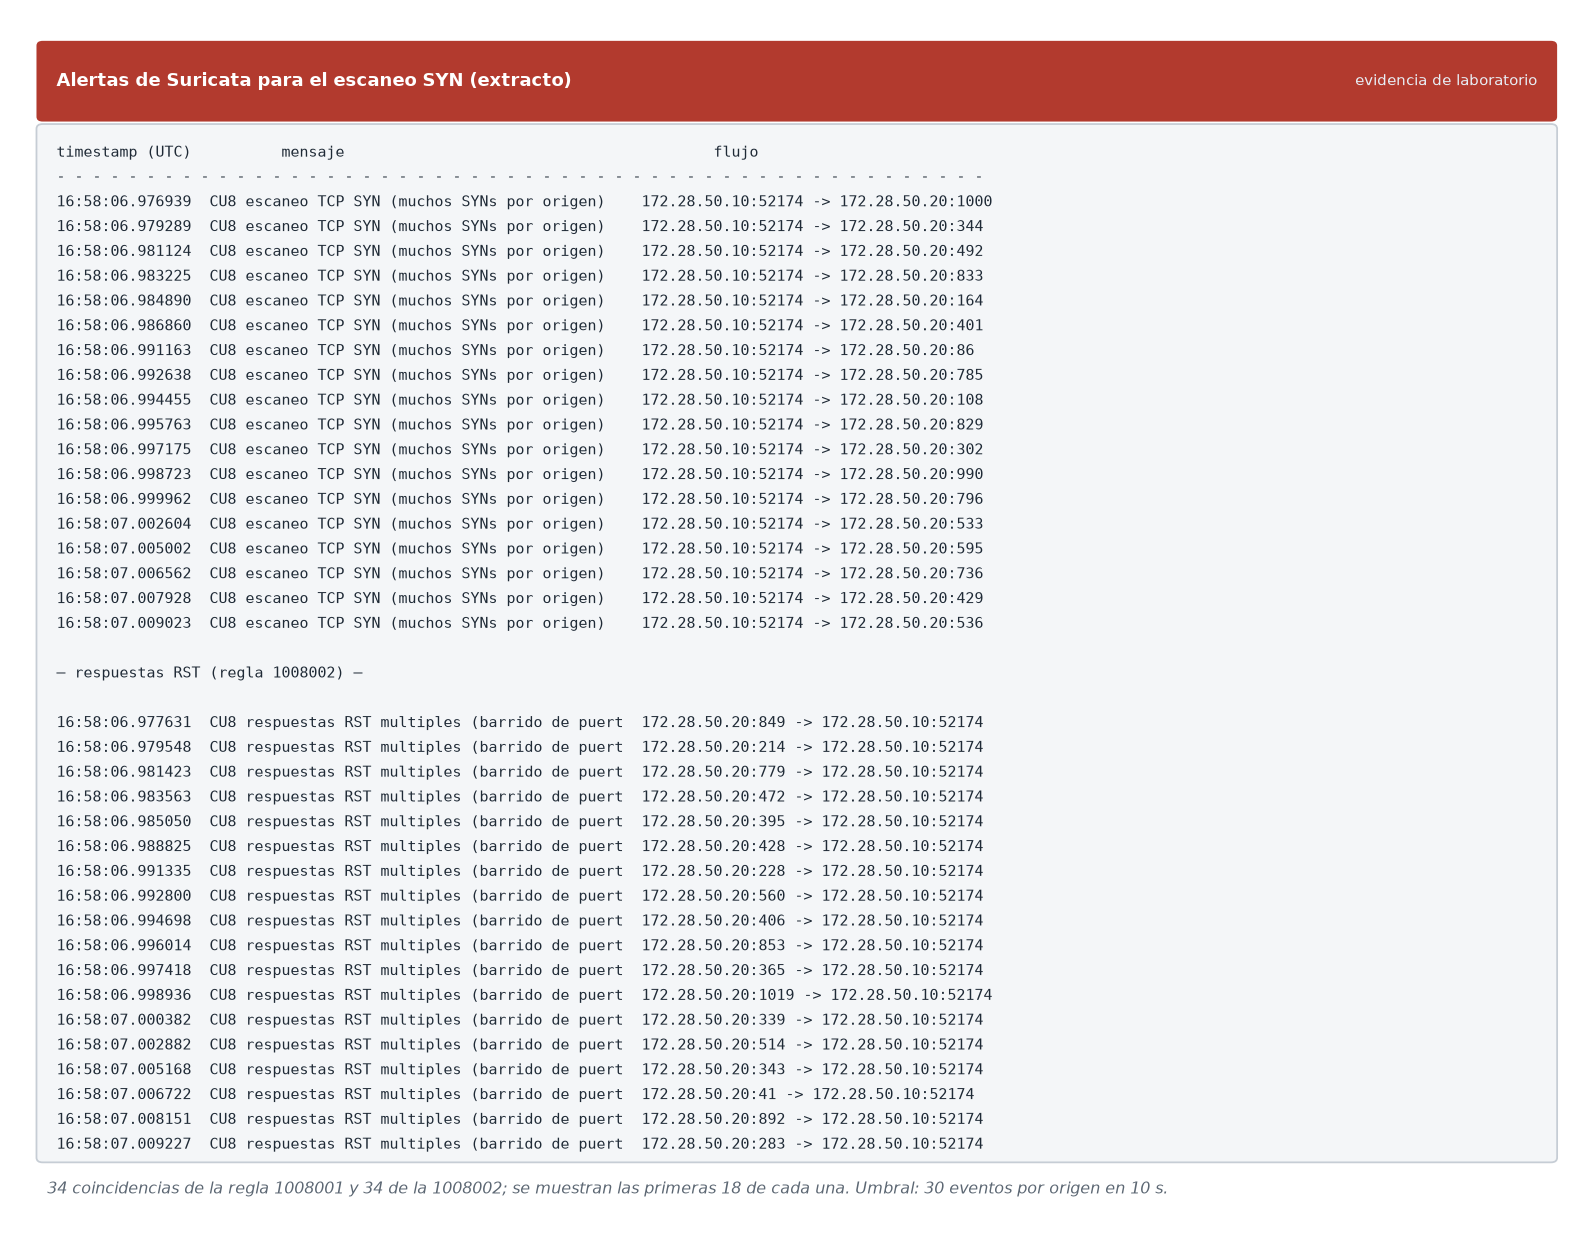
\includegraphics[width=0.98\textwidth]{imagenes/Evidencias CU-8/06_suricata_alertas.png}
	\caption{Alertas de Suricata 7.0.7 para el escaneo SYN (extracto de \texttt{fast.log}).}
	\label{fig:c8_suricata}
\end{figure}

\paragraph{Indicadores de detección.}
\begin{itemize}
	\item \textbf{Ráfaga de SYN:} más de 30 segmentos SYN desde un mismo origen en 10~s.
	\item \textbf{Barrido de puertos:} muchos puertos destino únicos y crecientes en un intervalo corto.
	\item \textbf{Relación SYN/RST:} predominio de RST sobre SYN-ACK, señal de puertos cerrados.
	\item \textbf{Fingerprinting:} conexiones completas seguidas de banners o cadenas de versión en varios puertos.
	\item \textbf{UDP e ICMP:} ráfaga de datagramas UDP con respuestas ICMP de puerto inalcanzable.
\end{itemize}

\paragraph{Regla de detección propuesta.}
Las reglas se validaron con Suricata: 34 alertas de la regla~1008001 y 34 de la regla~1008002 sobre \texttt{CU8\_01\_syn\_scan.pcap}. El umbral de 30 eventos por origen en 10~s evita que un cliente que abre varias conexiones normales dispare la alerta.

\begin{verbatim}
alert tcp 172.28.50.10 any -> 172.28.50.20 any (
  msg:"CU8 escaneo TCP SYN (muchos SYNs por origen)"; flags:S;
  threshold:type threshold, track by_src, count 30, seconds 10;
  classtype:attempted-recon; sid:1008001; rev:1;)

alert tcp 172.28.50.20 any -> 172.28.50.10 any (
  msg:"CU8 respuestas RST multiples (barrido de puertos)"; flags:R*;
  threshold:type threshold, track by_dst, count 30, seconds 10;
  classtype:attempted-recon; sid:1008002; rev:1;)
\end{verbatim}

\paragraph{Lista de exposición y endurecimiento.}
La Tabla~\ref{tab:exposicion} clasifica los servicios observados. La decisión de exposición debe justificarse por necesidad operativa y no por comodidad de instalación.

\begin{table}[H]
	\caption{Lista de exposición de servicios propios}
	\label{tab:exposicion}
	\centering
	\footnotesize
	\renewcommand{\arraystretch}{1.25}
	\begin{tabularx}{\textwidth}{@{}c >{\raggedright\arraybackslash}p{0.13\textwidth} >{\raggedright\arraybackslash}p{0.14\textwidth} c Y >{\raggedright\arraybackslash}p{0.18\textwidth}@{}}
		\toprule
		\textbf{Puerto} & \textbf{Servicio} & \textbf{Versión} & \textbf{¿Expuesto?} & \textbf{Justificación} & \textbf{Control propuesto} \\ \midrule
		21 & FTP & Laboratorio FTP 1.0 & Sí & Protocolo heredado sin cifrado. & Deshabilitar o migrar a SFTP/FTPS. \\ \hline
		22 & SSH & OpenSSH 9.7 & Sí & Administración remota. & Restringir por origen, solo claves y MFA. \\ \hline
		23 & Telnet & Laboratorio Telnet 0.9 & Sí & Credenciales en claro. & Deshabilitar de forma definitiva. \\ \hline
		80 & HTTP & nginx & Sí & Publicación web. & Redirigir a HTTPS y aplicar WAF. \\ \hline
		4444 & Desconocido & LAB-SVC/0.1 & Sí & Servicio de prueba sin justificación. & Cerrar salvo necesidad documentada. \\ \hline
		8080 & HTTP & LabHTTP/0.9 & Sí & Servicio de pruebas. & Restringir a la red de laboratorio. \\
		\bottomrule
	\end{tabularx}
\end{table}

\paragraph{Mitigación y defensa.}
\begin{itemize}
	\item \textbf{Reducción de superficie:} apagar servicios que no se usan y sustituir FTP/Telnet por SFTP/SSH.
	\item \textbf{Segmentación y firewall:} política de denegación por defecto y apertura solo desde redes y usuarios autorizados.
	\item \textbf{Control de tasa y bloqueo temporal:} limitar conexiones por origen y aplicar bloqueo con revisión ante barridos sostenidos.
	\item \textbf{Endurecimiento:} minimizar banners, actualizar versiones, usar TLS en los servicios publicados y revisar privilegios.
	\item \textbf{Monitorización:} correlacionar alertas de IDS con inventario de servicios y con ventanas de mantenimiento.
	\item \textbf{Pruebas autorizadas:} programar escaneos desde direcciones conocidas y documentarlos para separar el monitoreo legítimo de un ataque.
\end{itemize}

\paragraph{Preguntas de análisis.}
\begin{enumerate}
	\item \textbf{¿Qué limitaciones tiene atribuir un escaneo a una sola IP?}\par
	Una dirección IP no identifica de forma única a una persona o equipo: puede estar detrás de NAT o de un proxy, puede haber sido asignada por DHCP a otro host, puede estar suplantada mediante \textit{spoofing} o formar parte de una botnet distribuida. La atribución requiere correlacionar flujos, horarios, registros de autenticación, inventario de activos y, cuando exista, evidencia del proveedor; la IP por sí sola es solo un punto de partida.
	\item \textbf{¿Cómo se reducen los falsos positivos por monitoreo autorizado?}\par
	Con listas de escáneres autorizados, ventanas de mantenimiento, autenticación de los escaneos, umbrales calibrados con la línea base, supresión temporal con caducidad y correlación con el sistema de gestión de cambios. También ayuda distinguir el escaneo de inventario (puertos conocidos y periodicidad estable) del escaneo oportunista (puertos aleatorios y ráfaga anómala).
\end{enumerate}

\paragraph{Conclusiones.}
\begin{itemize}
	\item El escaneo SYN se detectó con precisión por la ráfaga de segmentos y la proporción de RST; las dos reglas de Suricata se validaron con 34 alertas cada una.
	\item El fingerprinting identificó versiones concretas y reveló un servicio no estándar en el puerto 4444 que no debería estar expuesto.
	\item El escaneo UDP mostró su ambigüedad inherente: la falta de respuesta no equivale a puerto abierto.
	\item La lista de exposición permite priorizar el cierre de FTP, Telnet y servicios de prueba, y restringir SSH y HTTP.
	\item Las limitaciones incluyen el tamaño reducido del laboratorio, la latencia casi nula de la red virtual y la ausencia de técnicas de evasión.
\end{itemize}

\begin{table}[H]
	\centering
	\caption{Ficha de registro del hallazgo. Caso 8}
	\footnotesize
	\renewcommand{\arraystretch}{1.2}
	\begin{tabularx}{\textwidth}{@{}>{\raggedright\arraybackslash}p{0.23\textwidth} Y@{}}
		\toprule
		\textbf{Campo} & \textbf{Registro} \\ \midrule
		Identificador & Caso 8 (escaneo de puertos), evidencias \texttt{01\_hashes\_sha256.png} a \texttt{06\_suricata\_alertas.png}. Analista: Yader Ibraldo Quiroga Torres. \\ \hline
		Fecha y hora & 10 de noviembre de 2026, 11:58 (UTC$-$5). \\ \hline
		Origen/destino & Analista \texttt{172.28.50.10} hacia la víctima \texttt{172.28.50.20}. \\ \hline
		Observación & Escaneo SYN de 1024 puertos en 59~ms, fingerprinting de seis servicios y escaneo UDP de cinco puertos. \\ \hline
		Hipótesis & Un escaneo de puertos produce una ráfaga de SYN con muchos puertos destino y una proporción alta de RST, y el fingerprinting genera banners identificables. \\ \hline
		Validación & \texttt{tshark} confirmó 1024 SYN, 4 SYN-ACK y 1020 RST; Suricata generó 34 alertas por SYN y 34 por RST. \\ \hline
		Severidad & Media: exposición de FTP, Telnet y un servicio no justificado en el puerto 4444. \\ \hline
		Acción & Cerrar servicios innecesarios, restringir SSH y HTTP, y mantener las reglas de detección con umbrales calibrados. \\ \hline
		Integridad & \texttt{CU8\_01}: \texttt{9fef801c\dots55130c} (SHA-256 truncado; el valor completo está en el Anexo~A). \\
		\bottomrule
	\end{tabularx}
\end{table}
